\documentclass[10pt]{article}
\usepackage{listings}
\usepackage{float}
\usepackage{graphicx}
\usepackage{bussproofs}

\floatstyle{boxed}
\restylefloat{figure}

\begin{document}
\title{A Proposal for FTL's New Scheduler}
\author{Eric Atkinson}
\maketitle

\section{Introduction}
The current scheduler for FTL is based on an enumerate-and-check algorithm that searches through possible schedules somewhat haphazardly and stops once it finds a valid one. It has the advantage of being easy to implement given a verification algorithm, but it is not able to explore the space of schedules in a principled way (which may be useful for building extensions to the FTL system). Also, the verification conditions are tricky to get right in all cases. This
proposal is for an alternative scheduler that operates more directly with the dependency graph, allowing it to explore the schedule space more thoroughly.

\section{The Dependency Graph}
Instead of a general algorithm for constructing the dependency graph from an attribute grammar, we will consider the motivating example shown in Figure~\ref{fig:grammar}. This grammar defines a set of trees whose nodes each have four attributes (except the root node, which has none). We would like to generate code that can compute all attributes for any tree in the set. However, the grammar defines some data dependencies that significantly impact this code's operation (e.g. we must
compute a Leaf's c attribute before we can compute its d attribute).

\begin{figure}[h]
    \lstinputlisting{example.ftl}
    \caption{Example grammar}
    \label{fig:grammar}
\end{figure}

We can begin constructing a dependency graph as follows: create a vertex for each $ (\textrm{class},\textrm{attribute}) $ combination, adding extra attributes for a class's children. Also, create an edge whenever there is a \emph{local} dependency between two attributes (these are dependencies we can ``read off the grammar''). This is shown in Figure~\ref{fig:local}.

\begin{figure}[h]
    \begin{center}
        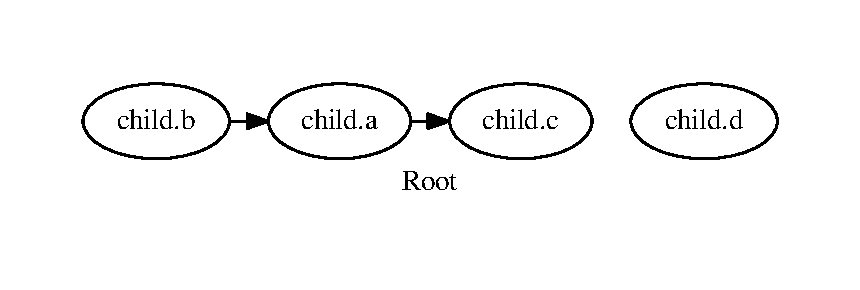
\includegraphics[scale=0.4]{root} \\
        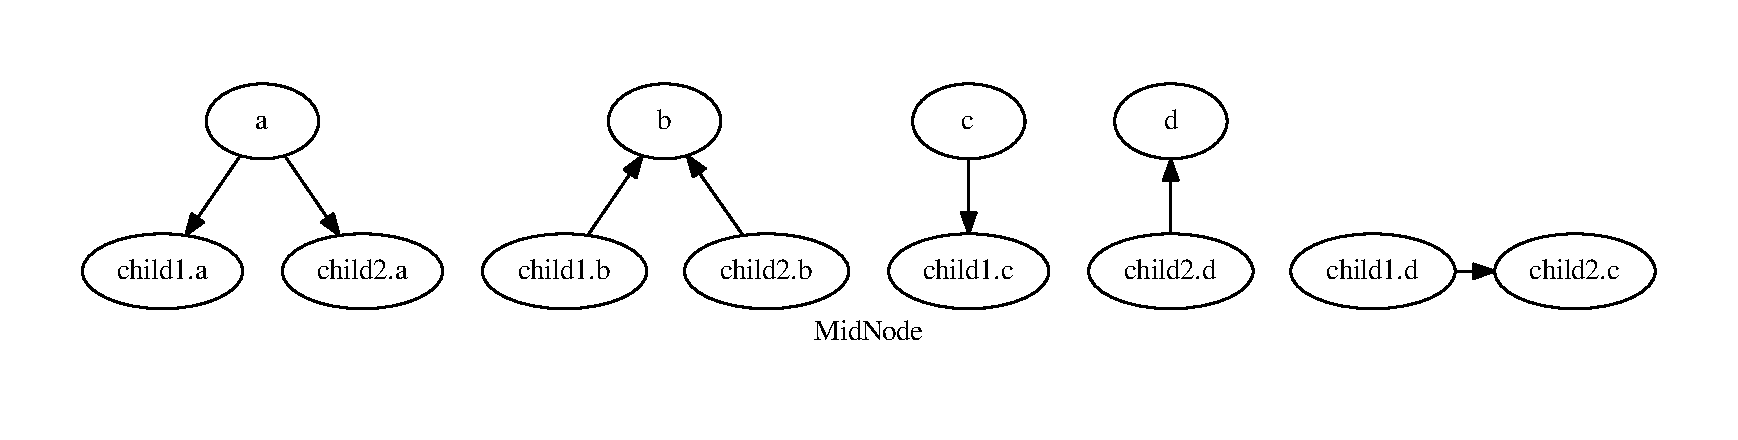
\includegraphics[scale=0.4]{midnode} \\
        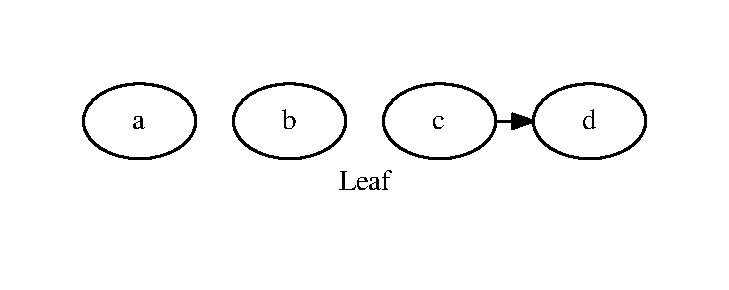
\includegraphics[scale=0.4]{leaf} \\
    \end{center}

    \caption{Local dependencies for the grammar in Figure~\ref{fig:grammar}}
    \label{fig:local}
\end{figure}

\begin{figure}[h]
    \begin{center}
        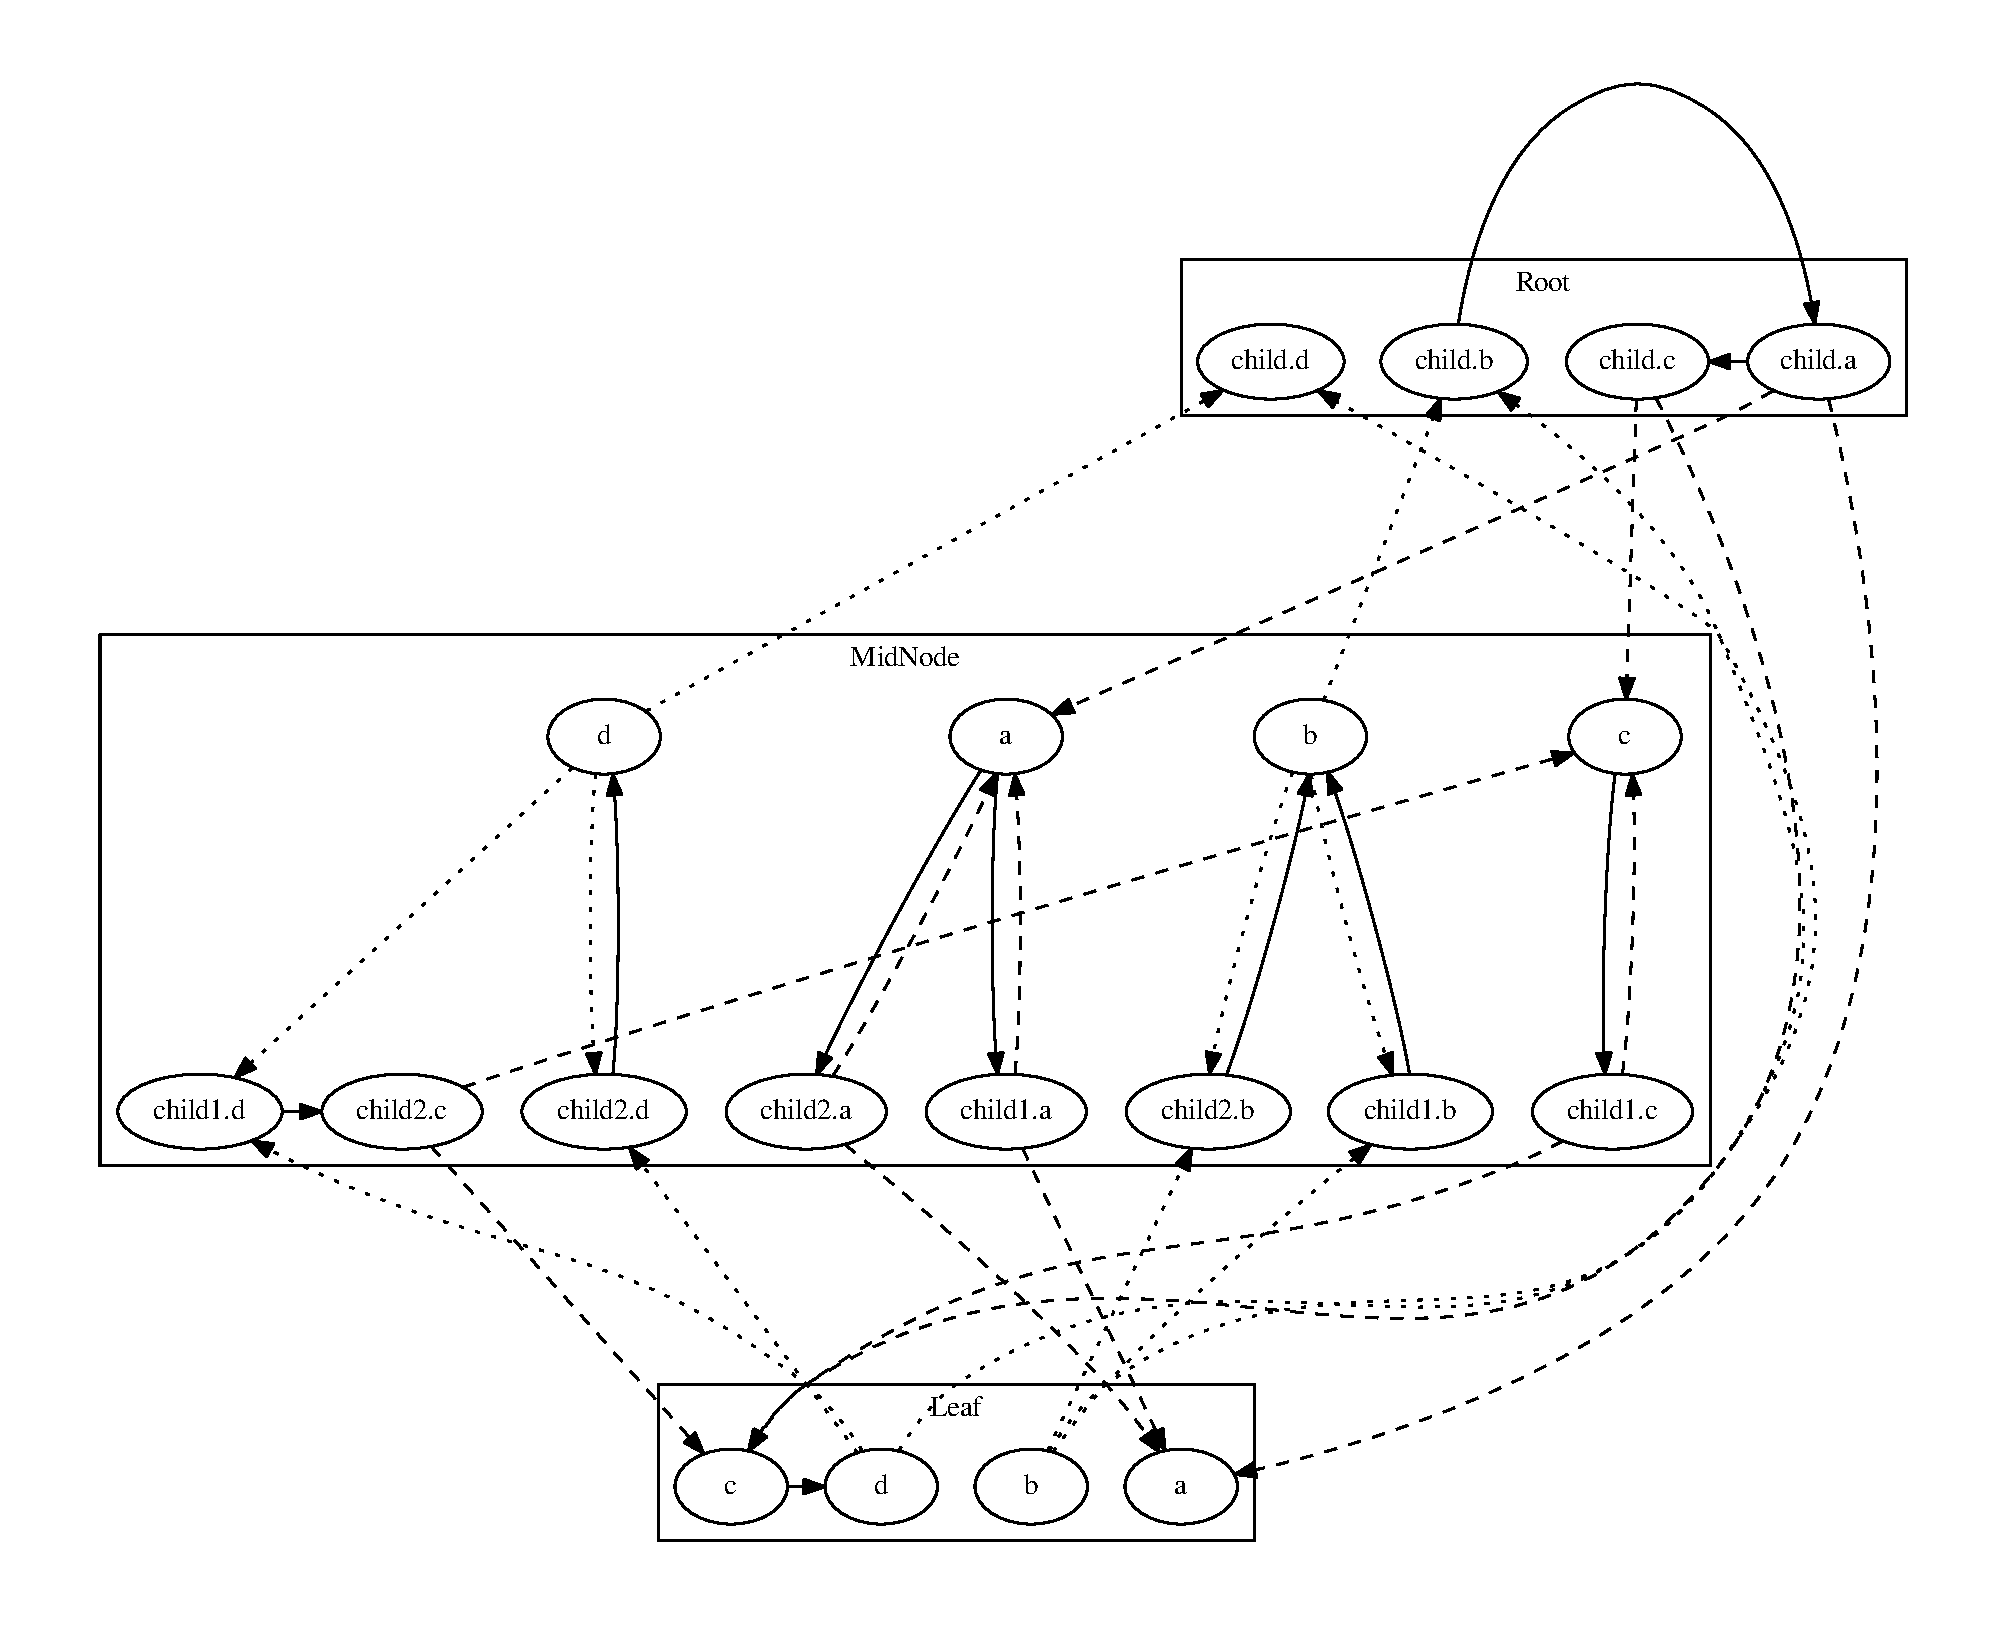
\includegraphics[scale=0.3]{complete}
    \end{center}
    \caption{Complete dependency graph for the grammar in Figure~\ref{fig:grammar}. Dotted lines represent sythesized dependencies, and dashed lines represent inherited dependencies}
    \label{fig:complete}
\end{figure}

As first observed by Knuth, we can obtain the dependency graph for any concrete tree by ``stitching'' together these local dependency graphs. The way we compose them is defined by the structure of the tree, which is not known at scheduling time. We assume instead that any valid ``stitching'' is possible. This means that, for example, if a class reads an attribute of its child, we need to add dependencies from \emph{any} class that child could possibly be. Figure~\ref{fig:complete}
adds these dependencies on top of the local ones already present in Figure~\ref{fig:local} to construct the complete dependency graph. It is also useful here to distinguish between \emph{inherited} and \emph{synthesized} dependencies. \emph{Inherited} dependencies are inter-class dependencies that flow from parents down to their children. \emph{Synthesized} dependencies are the reverse, flowing from children up to their parents.

\section{Scheduling}
Let $G = (V, E)$ be the complete dependency graph, as described in the previous section (here $V$ is the set of vertices and $E$ is the set of edges). Our goal is to produce a suitable \emph{traversal schedule} from this. A traversal $T$ in this context is simply a subgraph $T = (V_T, E_T)$, where $ V_T \subseteq V$ and $ E_T = \{(v_1,v_2) | (v_1, v_2) \in E \wedge  v_1,v_2 \in V_T\}$, that has some special properties. A \emph{traversal schedule} is a partition of $G$ such that each member of the
partition is a traversal.

\subsection{Traversal Properties}
To be a traversal, a subgraph $T = (V_T, E_T)$ must satisfy two conditions:
\begin{itemize}
    \item \textbf{Self Contained.} For any two verticies $v_1, v_2 \in V_T$, if $v_x \in V$ is on any path from $v_1$ to $v_2$, we must have $v_x \in V_T$. The reason we need this is to keep traversals ``contiguous''. If dependencies were allowed to wander out of traversals and back in again, we wouldn't be able to provide strong enough guarantees about when a vertex can be computed.
    \item \textbf{Traversable.} Each type of traversal makes assumptions about the order in which attributes are computed. The dependencies in $T$ must match these assumptions for at least one type of traversal. While the specifics are different for each type, these conditions generally take the form ``assume some subset of verticies $T$ can be computed; the remaining verticies of $T$ must be computable from these alone''.
\end{itemize}

The self contained property provides much insight into the space of possible traversal schedules. Note that for any two different verticies $v_1,v_2 \in S$, where $S$ is a strongly connected component of $G$, $v_2$ is on a path from $v_1$ to itself. This means that $v_1$ and $v_2$, or more generally all of $S$, must be on the same traversal. 

This suggests a novel way of discovering all possible traversal schedules. First, find all of the strongly connected components and assign them to traversals. These components now must form a DAG that is a valid \emph{traversal schedule}. We can construct other schedules by combining connected components together. While not always possible, in some cases we can continue this until the entire schedule is one big traversal. Hence the number of possible schedules is
$O(2^{|E_C|})$, where $E_C$ is the set of edges between the strongly connected components of $G$.

\subsection{Traversal Types}
We are interested in four different types of traversals, which each move around the tree in a different manner:
\begin{itemize}
    \item \textbf{Trivial} The trivial traversal imposes no restrictions on which order nodes of the tree may be visited in. A valid implementation strategy for this traversal is to visit all nodes in parallel.
    \item \textbf{Top Down} In a top down traversal, we visit a parent before visiting its children. 
    \item \textbf{Bottom Up} Bottom up traversals are exactly the reverse of top down ones. We visit all children of a node before visitng the node itself.
    \item \textbf{Inorder} On an inorder traversal, each child node is visited as part of some intermediate step of the parent visit. The parent can perform an arbitrary amount of computation before or after the visit, but each child is required to be visited exactly once.
\end{itemize}

To be traversable, we must be able to show that all nodes can be visited in one of these orders. This amounts to providing a proof that all vertices on the current traversal can be "computed". Usually, a vertex can be computed if all vertices it locally depends on can also be computed, but there are some special cases.

In general, we can assume that dependencies originating from outside the current traversal are always computable; we can presumably satisfy these by scheduling other traversals before the current one. For non-local dependencies within the current traversal, computability depends on which type of traversal we are considering. Below, we consider computability rules for two traversal types.

\begin{itemize}
    \item \textbf{Bottom Up} Assume that any synthesized dependencies are satisfied. If all verticies are computable from this alone (i.e. they have all dependencies satisfied), the traversal is bottom up.
    \item \textbf{Inorder} For a given class introduce a \emph{visit clause} for each one of its children. A \emph{visit clause} depends on all inherited dependencies to that child, and any synthesized dependencies from the child are satisfied iff the child's \emph{visit clause} is. Assuming all inherited dependencies are satisfied, if all vertices are computable, the traversal is inorder.
\end{itemize}

These conditions provide natural implementation strategies for each type of traversal. For example, with bottom-up traversals, once all of a node's children have been visited, any synthesized dependencies to the parent must have been satisfied, so we can immediately visit the parent and compute all of its attributes.

For inorder traversals, once we compute a child's inherited dependencies, we can visit that child and compute all of its attributes. This will satisfy any synthesized dependencies, allowing the parent to continue its visit.

Figures~\ref{fig:logic1} and~\ref{fig:logic2} lay out explicit logical rules for verifying a traversal is a particular type using only the dependency graph.
\begin{figure}
    \scriptsize
    \begin{prooftree}
        \AxiomC{$\forall e=(v_1,v_2) \in E, e $ is t-valid}
        \UnaryInfC{$v_2$ is t-computable}
    \end{prooftree}
    \begin{prooftree}
        \AxiomC{$e \not \in E_T$}
        \UnaryInfC{$e$ is t-valid}
    \end{prooftree}
    \begin{prooftree}
        \AxiomC{$e=(v_1,v_2) \in E_T$}
        \AxiomC{$e$ is local}
        \AxiomC{$v_1$ is t-computable}
        \TrinaryInfC{$e$ is t-valid}
    \end{prooftree}
    \begin{prooftree}
        \AxiomC{$\forall v \in V_T, v$ is t-computable}
        \UnaryInfC{$T$ is trivial}
    \end{prooftree}


    \begin{prooftree}
        \AxiomC{$\forall e=(v_1,v_2) \in E, e $ is td-valid}
        \UnaryInfC{$v_2$ is td-computable}
    \end{prooftree}
    \begin{prooftree}
        \AxiomC{$e \not \in E_T$}
        \UnaryInfC{$e$ is td-valid}
    \end{prooftree}
    \begin{prooftree}
        \AxiomC{$e \in E_T$}
        \AxiomC{$e$ is inherited}
        \BinaryInfC{$e$ is td-valid}
    \end{prooftree}
    \begin{prooftree}
        \AxiomC{$e=(v_1,v_2) \in E_T$}
        \AxiomC{$e$ is local}
        \AxiomC{$v_1$ is td-computable}
        \TrinaryInfC{$e$ is td-valid}
    \end{prooftree}
    \begin{prooftree}
        \AxiomC{$\forall v \in V_T, v$ is td-computable}
        \UnaryInfC{$T$ is top down}
    \end{prooftree}

    \caption{Rules to determine traversal types from the dependency graph for trivial and top down traversals}

    \label{fig:logic1}
\end{figure}
\begin{figure}
    \scriptsize
    \begin{prooftree}
        \AxiomC{$\forall e=(v_1,v_2) \in E, e $ is bu-valid}
        \UnaryInfC{$v_2$ is bu-computable}
    \end{prooftree}
    \begin{prooftree}
        \AxiomC{$e \not \in E_T$}
        \UnaryInfC{$e$ is bu-valid}
    \end{prooftree}
    \begin{prooftree}
        \AxiomC{$e \in E_T$}
        \AxiomC{$e$ is synthesized}
        \BinaryInfC{$e$ is bu-valid}
    \end{prooftree}
    \begin{prooftree}
        \AxiomC{$e=(v_1,v_2) \in E_T$}
        \AxiomC{$e$ is local}
        \AxiomC{$v_1$ is bu-computable}
        \TrinaryInfC{$e$ is bu-valid}
    \end{prooftree}
    \begin{prooftree}
        \AxiomC{$\forall v \in V_T, v$ is bu-computable}
        \UnaryInfC{$T$ is bottom up}
    \end{prooftree}


    \begin{prooftree}
        \AxiomC{$e \in E$}
        \AxiomC{$e \not \in E_T$}
        \BinaryInfC{$e$ is io-valid}
    \end{prooftree}
    \begin{prooftree}
        \AxiomC{$e \in E_T$}
        \AxiomC{$e$ is inherited}
        \BinaryInfC{$e$ is io-valid}
    \end{prooftree}
    \begin{prooftree}
        \AxiomC{$e = (v_1,v_2) \in E_T$}
        \AxiomC{$e$ is local}
        \AxiomC{$v_1$ is io-computable}
        \TrinaryInfC{$e$ is io-valid}
    \end{prooftree}
    \begin{prooftree}
        \AxiomC{$\forall (v_1,v_2) \in \{ e=(v_a, v_b) | v_a.class = c_1 \wedge v_b.class = c_2 \wedge e$ is inherited$ \}$}
        \AxiomC{$v_1$ is io-computable}
        \BinaryInfC{$visit(c_1,c_2)$}
    \end{prooftree}
    \begin{prooftree}
        \AxiomC{$e = (v_1,v_2) \in E_T$}
        \AxiomC{$e$ is synthesized}
        \AxiomC{$visit(v_1.class,v_2.class)$}
        \TrinaryInfC{$e$ is io-valid}
    \end{prooftree}
    \begin{prooftree}
        \AxiomC{$\forall (v_1,v_2) \in E, (v_1,v_2) $ is io-valid}
        \UnaryInfC{$v_2$ is io-computable}
    \end{prooftree}
    \begin{prooftree}
        \AxiomC{$\forall v \in V_T, v$ is io-computable}
        \UnaryInfC{$T$ is inorder}
    \end{prooftree}
    \caption{Rules to determine traversal types from the dependency graph for bottom up and inorder traversals}
    \label{fig:logic2}
\end{figure}

\subsection{Merging Traversals}
In some cases, two traversals can be merged into one. This is almost always neccessary after assigning traversals to strongly connected components because we wind up with the largest number of traversals possible, which is likely unsuitable for realistic implementations.

We define the merge of two traversals as follows: Let $T_1 = (V_1, E_1)$ and $T_2 = (V_2, E_2)$ be traversals. Their merge $T' = T_1 + T_2$ is such that $V_{T'} = V_1 \cup V_2$ and $E_{T'} = E_1 \cup E_2 \cup E_C$, where $E_C$ is the set of all edges across the cut between $T_1$ and $T_2$.

However, a merge is not always well defined. It only makes sense if the input traversals have specific types. Some of these type constraints are summarized below. These can be verified with the rules in Figures~\ref{fig:logic1} and~\ref{fig:logic2}, though the proofs are ommitted here.
\begin{itemize}
    \item If $T_1$ and $T_2$ are trivial, then $T'$ is trivial iff $E_C$ contains only local edges.
    \item If $T_1$ and $T_2$ are trivial, then $T'$ is bottom up iff $E_C$ contains no inherited edges.
    \item If $T_1$ and $T_2$ are trivial, then $T'$ is top down iff $E_C$ contains no synthesized edges.
    \item If $T_1$ and $T_2$ are top down, then $T'$ is top down iff $E_C$ contains no synthesized edges.
    \item If $T_1$ and $T_2$ are bottom up, then $T'$ is bottom up iff $E_C$ contains no inherited edges.
    \item If $T_1$ is top down and $T_2$ is inorder, then $T'$ is inorder iff $E_C$ contains no synthesized edges.
    \item If $T_1$ is inorder and $T_2$ is bottom up, then $T'$ is inorder iff $E_C$ contains no synthesized edges.

\end{itemize}
\end{document}
